\documentclass[11pt,a4paper]{article}

\usepackage[margin=2.4cm,top=2.6cm,bottom=2.6cm]{geometry}
\usepackage{amsmath,amssymb,mathtools}
\usepackage{siunitx}
\usepackage{booktabs,tabularx,array}
\usepackage[dvipsnames,svgnames]{xcolor}
\usepackage{tikz}
\usepackage{circuitikz}
\usepackage{pgfplots}
\usepackage[most]{tcolorbox}
\usepackage{titlesec}
\usepackage{enumitem}
\usepackage{caption}
\usepackage{microtype}
\usepackage[hidelinks]{hyperref}

\pgfplotsset{compat=1.18}
\usetikzlibrary{arrows.meta,positioning,calc,decorations.pathmorphing,decorations.markings,patterns,shapes.geometric}

% ---------- palette, matched to the web edition ----------
\definecolor{ink}{HTML}{17201D}
\definecolor{paper}{HTML}{F3F0E7}
\definecolor{deep}{HTML}{25483D}
\definecolor{mint}{HTML}{9BC9B3}
\definecolor{gold}{HTML}{C49A54}
\definecolor{sig}{HTML}{5AA9C8}
\definecolor{hot}{HTML}{C2685A}
\definecolor{rule}{HTML}{B7B2A6}

\color{ink}
\sisetup{detect-all,per-mode=symbol,group-separator={\,}}
\DeclareSIUnit{\ppm}{ppm}
\DeclareSIUnit{\rpm}{rpm}
\DeclareSIUnit{\vph}{vph}
\DeclareSIUnit{\mnth}{month}

\titleformat{\section}{\Large\bfseries\color{deep}}{\thesection}{0.8em}{}
\titleformat{\subsection}{\large\bfseries\color{ink}}{\thesubsection}{0.7em}{}
\titlespacing*{\section}{0pt}{2.2ex plus 1ex minus .2ex}{1.2ex plus .2ex}

\newtcolorbox{keybox}[1][]{colback=paper,colframe=gold,boxrule=0pt,
  leftrule=3pt,arc=0pt,left=10pt,right=10pt,top=8pt,bottom=8pt,#1}

\captionsetup{font=small,labelfont={bf,color=deep},width=.92\textwidth}

\newcommand{\lab}[1]{{\footnotesize\sffamily #1}}

\title{\vspace{-1.6cm}\color{deep}\Huge Inside a Quartz Watch\\[2mm]
\normalsize\color{ink}\normalfont
From a piezoelectric tuning fork to a stepping seconds hand}
\author{}
\date{}

\begin{document}
\maketitle
\vspace{-1.4cm}

\begin{center}
\rule{\textwidth}{0.6pt}
\end{center}

\noindent\emph{Companion to the interactive edition at
\texttt{theisegoria.github.io/quartz-lab/}, and to the automatic-watch lab at
\texttt{theisegoria.github.io/watch-lab/}. Component values, currents and ratios
throughout are typical rather than specific to any one calibre.}

\vspace{4mm}

\section*{The argument in one paragraph}
\addcontentsline{toc}{section}{The argument in one paragraph}

A mechanical watch \emph{measures}. Energy enters an escapement, a balance wheel answers with
an interval, and every imperfection in that negotiation appears as rate. A quartz watch
\emph{counts}. A laser-trimmed sliver of silicon dioxide vibrates \SI{32768}{\hertz}, fifteen
toggle flip-flops halve that number down to exactly \SI{1}{\hertz}, and the single pulse left
over is spent turning a magnet through half a revolution. Nothing downstream of the crystal is
allowed to influence the rate. That structural fact, rather than the raw frequency, is what
makes quartz timekeeping a different category rather than a better version of the same thing.

\tableofcontents

\vspace{4mm}

% ==================================================================
\section{The signal path}

\begin{figure}[htbp]
\centering
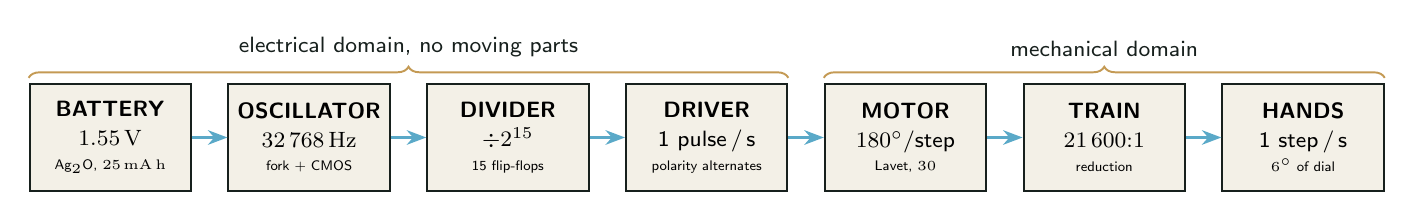
\begin{tikzpicture}[
  font=\footnotesize\sffamily,
  box/.style={draw=ink,line width=.7pt,minimum width=2.05cm,minimum height=1.35cm,
              align=center,fill=paper,inner sep=2pt},
  >=Stealth]
\node[box] (b)                        {\textbf{BATTERY}\\[1pt]\SI{1.55}{\volt}\\[-1pt]\tiny Ag$_2$O, \SI{25}{\milli\ampere\hour}};
\node[box,right=4.5mm of b]  (o)      {\textbf{OSCILLATOR}\\[1pt]\SI{32768}{\hertz}\\[-1pt]\tiny fork + CMOS};
\node[box,right=4.5mm of o]  (d)      {\textbf{DIVIDER}\\[1pt]$\div 2^{15}$\\[-1pt]\tiny 15 flip-flops};
\node[box,right=4.5mm of d]  (r)      {\textbf{DRIVER}\\[1pt]1 pulse\,/\,s\\[-1pt]\tiny polarity alternates};
\node[box,right=4.5mm of r]  (m)      {\textbf{MOTOR}\\[1pt]$180^\circ$/step\\[-1pt]\tiny Lavet, \SI{30}{\rpm}};
\node[box,right=4.5mm of m]  (t)      {\textbf{TRAIN}\\[1pt]$21\,600{:}1$\\[-1pt]\tiny reduction};
\node[box,right=4.5mm of t]  (h)      {\textbf{HANDS}\\[1pt]1 step\,/\,s\\[-1pt]\tiny $6^\circ$ of dial};
\foreach \a/\b in {b/o,o/d,d/r,r/m,m/t,t/h}
  \draw[->,line width=.9pt,sig] (\a) -- (\b);
\draw[decorate,decoration={brace,amplitude=4pt,raise=2pt},gold,line width=.7pt]
  (b.north west) -- (r.north east) node[midway,above=6pt,ink]{electrical domain, no moving parts};
\draw[decorate,decoration={brace,amplitude=4pt,raise=2pt},gold,line width=.7pt]
  (m.north west) -- (h.north east) node[midway,above=6pt,ink]{mechanical domain};
\end{tikzpicture}
\caption{Seven stages. Everything left of the motor is electronics; everything right of it is a
watch in the ordinary sense. Total draw is about \SI{1.3}{\micro\ampere}, of which the motor
takes roughly \SI{0.5}{\micro\ampere}, about as much as all of the silicon put together.}
\end{figure}

\begin{keybox}
\textbf{Power budget.} Oscillator \SI{0.3}{\micro\ampere}, divider and logic
\SI{0.5}{\micro\ampere}, motor pulses \SI{0.5}{\micro\ampere}. From a \SI{25}{\milli\ampere\hour}
silver-oxide cell that is roughly \SI{19000}{\hour}, or a little over two years. The cell's
voltage stays nearly flat until it collapses, which is why a quartz watch keeps perfect time
right up to the moment it stops.
\end{keybox}

% ==================================================================
\section{The resonator}

\subsection{Why quartz is piezoelectric}

$\alpha$-quartz belongs to trigonal crystal class 32, which has no centre of symmetry. Strain
displaces the Si$^{4+}$ and O$^{2-}$ sublattices by different amounts, so a deformed crystal
carries a net dipole and therefore a surface charge. The converse effect is what drives the
resonator: electrodes patterned along each tine apply a field that makes one face of the tine
extend and the other contract, and a bar that lengthens on one face and shortens on the other
bends. The same electrodes then read back the charge generated by that bending, which closes
the feedback loop. The crystal is simultaneously the actuator and the sensor.

\subsection{The flexural mode, and why antiphase matters}

\begin{figure}[htbp]
\centering
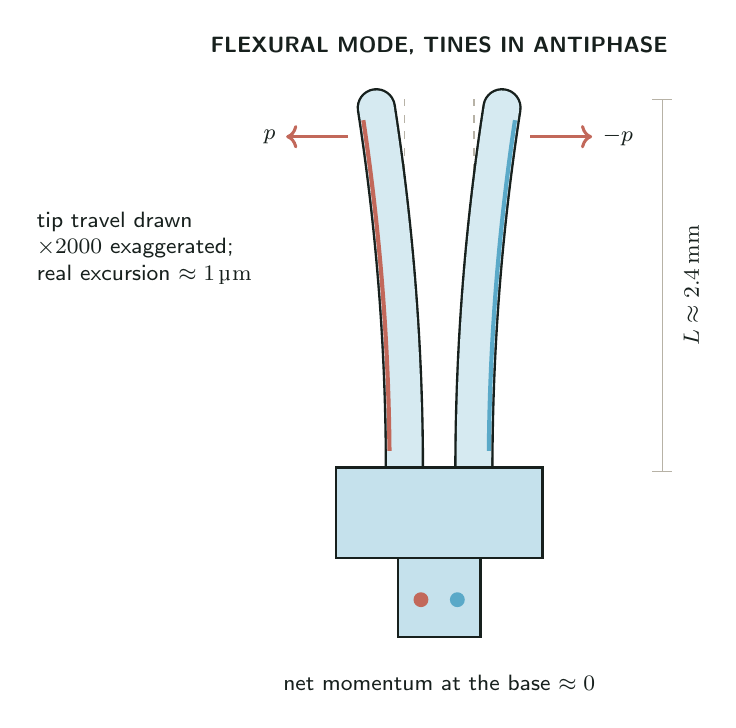
\begin{tikzpicture}[scale=1.05,font=\footnotesize\sffamily]
\def\bendL{plot[smooth,domain=0.02:4.4,samples=40] ({-0.42-0.34*(\x/4.4)*(\x/4.4)},\x)}
\def\bendR{plot[smooth,domain=0.02:4.4,samples=40] ({ 0.42+0.34*(\x/4.4)*(\x/4.4)},\x)}
\def\elL{plot[smooth,domain=0.25:4.25,samples=30] ({-0.60-0.34*(\x/4.4)*(\x/4.4)},\x)}
\def\elR{plot[smooth,domain=0.25:4.25,samples=30] ({ 0.60+0.34*(\x/4.4)*(\x/4.4)},\x)}
% neutral reference
\draw[rule,dashed,line width=.5pt] (-0.42,0) -- (-0.42,4.5);
\draw[rule,dashed,line width=.5pt] ( 0.42,0) -- ( 0.42,4.5);
% tine bodies
\draw[line width=0.50cm,ink,line cap=round] \bendL;
\draw[line width=0.44cm,sig!25,line cap=round] \bendL;
\draw[line width=0.50cm,ink,line cap=round] \bendR;
\draw[line width=0.44cm,sig!25,line cap=round] \bendR;
% electrodes
\draw[hot,line width=1.5pt] \elL;
\draw[sig,line width=1.5pt] \elR;
% base and stem
\fill[sig!35,draw=ink,line width=.8pt] (-1.25,-1.05) rectangle (1.25,0.05);
\fill[sig!35,draw=ink,line width=.8pt] (-0.50,-2.00) rectangle (0.50,-1.05);
\fill[hot] (-0.22,-1.55) circle (0.09);
\fill[sig] ( 0.22,-1.55) circle (0.09);
% momentum arrows
\draw[->,hot,line width=1.1pt] (-1.10,4.05) -- (-1.85,4.05) node[left,ink]{$p$};
\draw[->,hot,line width=1.1pt] ( 1.10,4.05) -- ( 1.85,4.05) node[right,ink]{$-p$};
% dimension
\draw[rule,line width=.5pt] (2.7,0) -- (2.7,4.5);
\draw[rule,line width=.5pt] (2.58,0) -- (2.82,0);
\draw[rule,line width=.5pt] (2.58,4.5) -- (2.82,4.5);
\node[rotate=90,ink] at (3.05,2.25) {$L \approx \SI{2.4}{\milli\metre}$};
\node[ink,align=left,anchor=east] at (-2.15,2.7)
  {tip travel drawn\\$\times 2000$ exaggerated;\\real excursion $\approx \SI{1}{\micro\metre}$};
\node[ink,align=center] at (0,-2.55) {net momentum at the base $\approx 0$};
\node[ink] at (0,5.15) {\textbf{FLEXURAL MODE, TINES IN ANTIPHASE}};
\end{tikzpicture}
\caption{The two tines carry equal and opposite momentum, so the reaction forces cancel where
the fork meets its mount. Almost nothing leaks out, which is why $Q$ reaches $10^4$ to $10^5$.
Drive the tines in phase instead and the base shakes, energy escapes, and the resonance
collapses.}
\end{figure}

For a flexural tine the resonant frequency follows the cantilever result
\begin{equation}
f \;\approx\; \frac{\beta_1^{2}}{2\pi}\,\frac{t}{L^{2}}\sqrt{\frac{E}{12\rho}}
  \;\approx\; 0.162\,\frac{t}{L^{2}}\sqrt{\frac{E}{\rho}},
  \qquad \beta_1 = 1.8751 ,
\label{eq:tine}
\end{equation}
so frequency scales with tine thickness and with the \emph{inverse square} of tine length.
With $E \approx \SI{78}{\giga\pascal}$ and $\rho = \SI{2650}{\kilogram\per\cubic\metre}$, a tine
roughly \SI{2.4}{\milli\metre} long and \SI{0.1}{\milli\metre} thick lands near
\SI{32}{\kilo\hertz}. The forks are photolithographically etched to micron tolerances and then
finished by laser: ablate gold from the tine tips and the frequency rises, deposit gold and it
falls, a few parts per million per pass. The tips are chosen because the mode shape has
maximum displacement there and therefore maximum mass sensitivity.

\begin{keybox}
\textbf{Why \num{32768} and not \num{100000}.} It is $2^{15}$, so fifteen halvings land exactly
on \SI{1}{\hertz} using nothing but toggle flip-flops. It is also a sweet spot for power: CMOS
dynamic power goes as $CV^{2}f$, so a higher-frequency crystal buys short-term stability at a
linear cost in battery life.
\end{keybox}

% ==================================================================
\section{The crystal as a circuit}

To the electronics the fork looks like the Butterworth--Van Dyke network of
Figure~\ref{fig:bvd}: a \emph{motional} branch $L_1 C_1 R_1$ in parallel with $C_0$, the static
capacitance of the electrodes and can.

\begin{figure}[htbp]
\centering
\begin{circuitikz}[american,scale=0.95,transform shape,font=\small]
  \draw (0,0) to[short,o-*] (1,0);
  \draw (1,0) -- (1,1.4) to[C=$C_0$,a=\lab{\SI{1.4}{\pico\farad}}] (5,1.4) -- (5,0);
  \draw (1,0) -- (1,-1.4)
        to[L=$L_1$,a_=\lab{\SI{7863}{\henry}}] (2.4,-1.4)
        to[C=$C_1$,a_=\lab{\SI{3.0}{\femto\farad}}] (3.6,-1.4)
        to[R=$R_1$,a_=\lab{\SI{30}{\kilo\ohm}}] (5,-1.4) -- (5,0);
  \draw (5,0) to[short,*-o] (6,0);
\end{circuitikz}
\caption{The Butterworth--Van Dyke equivalent circuit. $L_1$ is not an inductor: it is the
\emph{mass} of the vibrating tines expressed in electrical units, because a series $LCR$ and a
mass--spring--damper obey the same second-order equation. $C_1$ is the tine stiffness and $R_1$
is every loss mechanism added together. $Q = \omega L_1 / R_1 \approx \num{54000}$.}
\label{fig:bvd}
\end{figure}

The network has two resonances, series and parallel,
\begin{equation}
f_s = \frac{1}{2\pi\sqrt{L_1 C_1}},
\qquad
f_p = f_s\sqrt{1 + \frac{C_1}{C_0}} \;\approx\; f_s\!\left(1 + \frac{C_1}{2C_0}\right),
\end{equation}
and with a load capacitance $C_L$ presented by the oscillator the operating point sits at
\begin{equation}
f_L = f_s\!\left(1 + \frac{C_1}{2\,(C_0 + C_L)}\right).
\label{eq:pull}
\end{equation}

\begin{figure}[htbp]
\centering
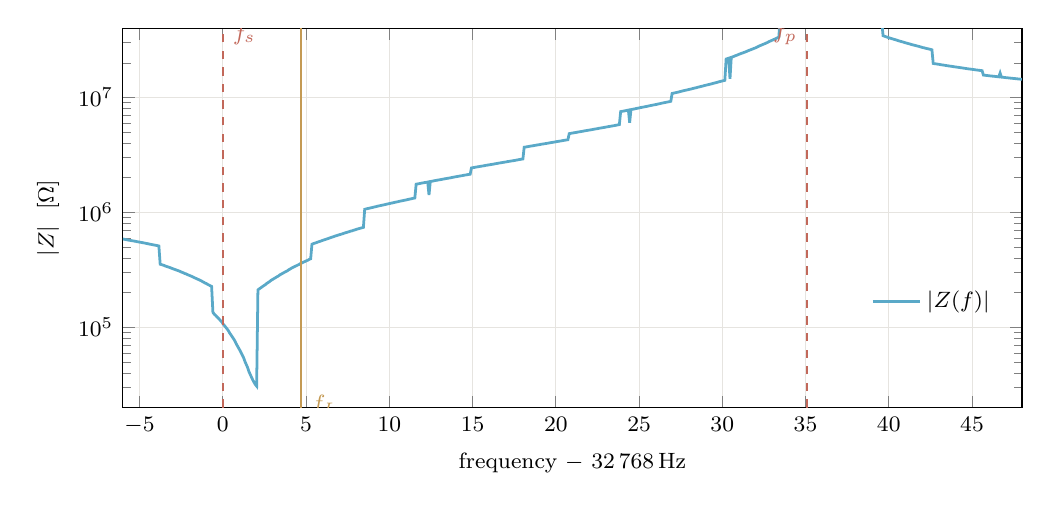
\begin{tikzpicture}
\begin{semilogyaxis}[
  width=13cm,height=6.4cm,
  xlabel={frequency $-\ \SI{32768}{\hertz}$},
  ylabel={$|Z|$\ \ [$\Omega$]},
  xmin=-6,xmax=48,ymin=2e4,ymax=4e7,
  grid=major,grid style={rule!35,very thin},
  tick label style={font=\footnotesize},
  label style={font=\footnotesize},
  every axis plot/.append style={line width=1pt},
  legend style={font=\footnotesize,draw=none,fill=none,at={(0.98,0.28)},anchor=east}]
  % |Z| of BVD with fs = 32768, C1 = 3fF, C0 = 1.4pF, R1 = 30k
  \addplot[sig,samples=700,domain=-6:48]
    {sqrt( ( (30000)^2 + (2*pi*(32768+x)*7863 - 1/(2*pi*(32768+x)*3e-15))^2 )
         / ( 1 + (2*pi*(32768+x)*1.4e-12)^2*((30000)^2 + (2*pi*(32768+x)*7863 - 1/(2*pi*(32768+x)*3e-15))^2)
             - 2*(2*pi*(32768+x)*1.4e-12)*(2*pi*(32768+x)*7863 - 1/(2*pi*(32768+x)*3e-15)) ) )};
  \addlegendentry{$|Z(f)|$}
  \draw[hot,dashed,line width=.8pt] (axis cs:0,2e4) -- (axis cs:0,4e7)
        node[pos=.93,above right,font=\footnotesize,hot]{$f_s$};
  \draw[hot,dashed,line width=.8pt] (axis cs:35.1,2e4) -- (axis cs:35.1,4e7)
        node[pos=.93,above left,font=\footnotesize,hot]{$f_p$};
  \draw[gold,line width=1pt] (axis cs:4.7,2e4) -- (axis cs:4.7,4e7)
        node[pos=.06,below right,font=\footnotesize,gold]{$f_L$};
\end{semilogyaxis}
\end{tikzpicture}
\caption{Impedance of the crystal against frequency. The deep minimum at $f_s$ equals $R_1$;
the sharp maximum at $f_p$ sits about \SI{35}{\hertz} higher, roughly \num{1070} parts per
million. The circuit can only pull the frequency inside that window, and in practice only
across the small part of it selected by $C_L$.}
\end{figure}

\begin{keybox}
\textbf{The gap is the stability.} Sliding $C_L$ from \SI{4}{\pico\farad} to
\SI{20}{\pico\farad} moves the operating point by roughly \SI{200}{\ppm}: about nine minutes a
month of adjustment authority, and that is the \emph{entire} regulation range of a quartz
watch. Compare a balance wheel, whose rate moves with amplitude, position and mainspring
torque. The crystal simply refuses to run anywhere else.
\end{keybox}

% ==================================================================
\section{Sustaining the vibration}

\begin{figure}[htbp]
\centering
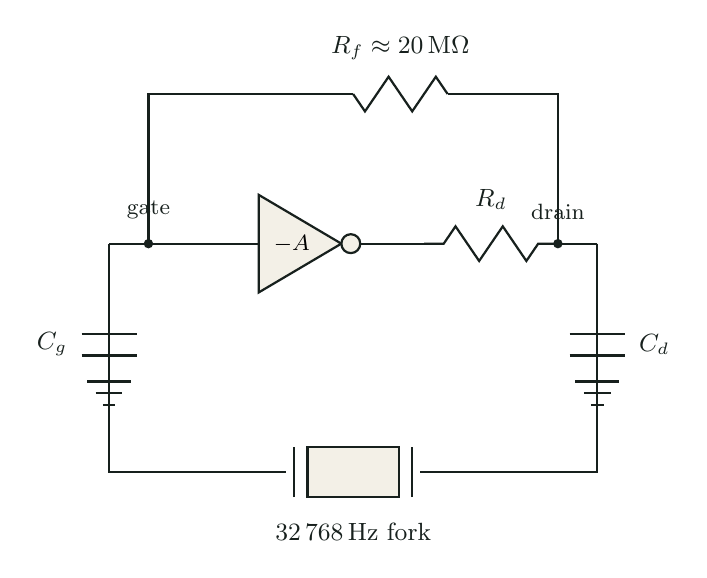
\begin{tikzpicture}[font=\small,>=Stealth,line width=.8pt,x=1cm,y=1cm]
% inverter
\draw[fill=paper,draw=ink] (3.0,0) -- (3.0,0.62) -- (4.05,0) -- (3.0,-0.62) -- cycle;
\draw[fill=paper,draw=ink] (4.17,0) circle (0.12);
\node at (3.42,0) {\footnotesize $-A$};
% main wire
\draw[ink] (1.6,0) -- (3.0,0);
\draw[ink] (4.29,0) -- (5.1,0);
% Rd
\draw[ink] (5.1,0) -- (5.35,0) -- (5.5,0.22) -- (5.8,-0.22) -- (6.1,0.22) -- (6.4,-0.22) -- (6.55,0) -- (6.8,0);
\node[above,ink] at (5.95,0.3) {$R_d$};
% feedback Rf
\draw[ink] (6.8,0) -- (6.8,1.9) -- (5.4,1.9);
\draw[ink] (5.4,1.9) -- (5.25,2.12) -- (4.95,1.68) -- (4.65,2.12) -- (4.35,1.68) -- (4.2,1.9);
\draw[ink] (4.2,1.9) -- (1.6,1.9) -- (1.6,0);
\node[above,ink] at (4.8,2.2) {$R_f \approx \SI{20}{\mega\ohm}$};
% Cg
\draw[ink] (1.1,0) -- (1.6,0);
\draw[ink] (1.1,0) -- (1.1,-1.15);
\draw[ink] (0.75,-1.15) -- (1.45,-1.15);
\draw[ink] (0.75,-1.42) -- (1.45,-1.42);
\draw[ink] (1.1,-1.42) -- (1.1,-1.75);
\draw[ink] (0.82,-1.75) -- (1.38,-1.75); \draw[ink] (0.93,-1.9) -- (1.27,-1.9); \draw[ink] (1.02,-2.05) -- (1.18,-2.05);
\node[left,ink] at (0.7,-1.28) {$C_g$};
% Cd
\draw[ink] (6.8,0) -- (7.3,0);
\draw[ink] (7.3,0) -- (7.3,-1.15);
\draw[ink] (6.95,-1.15) -- (7.65,-1.15);
\draw[ink] (6.95,-1.42) -- (7.65,-1.42);
\draw[ink] (7.3,-1.42) -- (7.3,-1.75);
\draw[ink] (7.02,-1.75) -- (7.58,-1.75); \draw[ink] (7.13,-1.9) -- (7.47,-1.9); \draw[ink] (7.22,-2.05) -- (7.38,-2.05);
\node[right,ink] at (7.7,-1.28) {$C_d$};
% crystal
\draw[ink] (1.1,0) -- (1.1,-2.9) -- (3.35,-2.9);
\draw[ink] (7.3,0) -- (7.3,-2.9) -- (5.05,-2.9);
\draw[fill=paper,draw=ink] (3.62,-3.22) rectangle (4.78,-2.58);
\draw[ink] (3.45,-3.22) -- (3.45,-2.58);
\draw[ink] (4.95,-3.22) -- (4.95,-2.58);
\node[below,ink] at (4.2,-3.42) {\SI{32768}{\hertz} fork};
% node labels
\fill[ink] (1.6,0) circle (0.06); \fill[ink] (6.8,0) circle (0.06);
\node[above,ink,font=\footnotesize] at (1.6,0.18) {gate};
\node[above,ink,font=\footnotesize] at (6.8,0.18) {drain};
\end{tikzpicture}
\caption{The CMOS Pierce oscillator. The inverter contributes $180^\circ$ of phase shift and
the $\pi$-network of $C_g$, the crystal and $C_d$ contributes another $180^\circ$; with loop
gain above unity the circuit has no choice but to oscillate. $R_f$ biases the inverter into its
own linear region, and $R_d$ limits how hard the fork is driven.}
\end{figure}

The tidiest way to see the circuit is that the inverter and its two capacitors present a
\emph{negative resistance} to the crystal,
\begin{equation}
R_{\mathrm{neg}} \;=\; -\,\frac{g_m}{\omega^{2} C_g C_d},
\end{equation}
and oscillation grows whenever $|R_{\mathrm{neg}}| > R_1$. With $g_m = \SI{1}{\micro\siemens}$
and $C_g = C_d = \SI{12}{\pico\farad}$ this is about \SI{-164}{\kilo\ohm}, a margin of roughly
$5.5\times$ over $R_1$. Designers want three to five times and no more: excess margin wastes
current and overdrives the fork.

Amplitude then grows from thermal noise as $e^{t/\tau}$ with
\begin{equation}
\tau \;=\; \frac{2 L_1}{|R_{\mathrm{neg}}| - R_1} \;\approx\; \SI{0.12}{\second},
\end{equation}
so full amplitude arrives after roughly half a second. The same enormous $L_1$ that makes the
fork stable makes it slow to wake: a high-$Q$ resonator is a flywheel, hard to disturb and
equally hard to spin up. Drive level matters at the other end of the scale, because overdrive
causes non-linear bending, accelerated ageing and, in extreme cases, fracture at the tine
roots. Watch crystals run at well under a microwatt.

% ==================================================================
\section{Counting down}

Fifteen toggle flip-flops, that is D flip-flops with the inverted output wired back to the input,
each change state once per two input cycles:
\[
\SI{32768}{\hertz} \xrightarrow{\ \div 2\ } \num{16384} \xrightarrow{\ \div 2\ } \num{8192}
\ \cdots\ \xrightarrow{\ \div 2\ } \num{2} \xrightarrow{\ \div 2\ } \SI{1}{\hertz}.
\]

\begin{figure}[htbp]
\centering
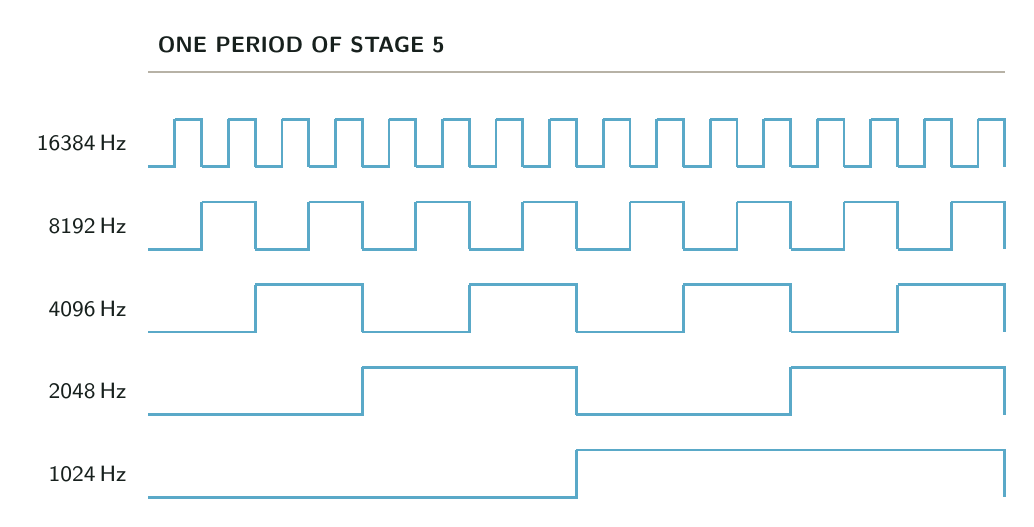
\begin{tikzpicture}[font=\footnotesize\sffamily,x=1cm,y=1cm]
\foreach \k/\lbl in {1/16384,2/8192,3/4096,4/2048,5/1024}{
  \pgfmathsetmacro{\yy}{-1.05*\k}
  \pgfmathsetmacro{\per}{2^\k}
  \node[anchor=east,ink] at (-0.15,\yy+0.3) {\lbl\,Hz};
  \draw[sig,line width=1pt]
    \foreach \n in {0,...,31}{
      (0.34*\n, {\yy + 0.6*mod(floor(\n/(\per/2)),2)}) --
      (0.34*\n+0.34, {\yy + 0.6*mod(floor(\n/(\per/2)),2)}) --
      (0.34*\n+0.34, {\yy + 0.6*mod(floor((\n+1)/(\per/2)),2)})
    };
}
\draw[rule,line width=.5pt] (0,0.15) -- (10.88,0.15);
\node[anchor=west,ink] at (0,0.5) {\textbf{ONE PERIOD OF STAGE 5}};
\end{tikzpicture}
\caption{The first five stages of the divider over one period of the fifth. Every stage is a
perfect \SI{50}{\percent} square wave and the edges never drift relative to one another:
division by two is exact in a way that no analogue process is, with no error term to
accumulate.}
\end{figure}

Two practical notes. First, dynamic power is $CV^2 f$ per stage and $f$ halves each time, so
the whole chain costs about twice what stage one costs; designers shrink the first flip-flop
and let the rest be lazy. Second, the motor does not want a \SI{50}{\percent} duty cycle at
\SI{1}{\hertz}. It wants a \SIrange{4}{8}{\milli\second} kick, so the driver gates a fast stage
(say \SI{256}{\hertz}) with the \SI{1}{\hertz} stage to cut a short pulse, then alternates its
polarity every second.

% ==================================================================
\section{The Lavet stepper motor}

This is the most-manufactured electric motor in the world, and the only place in a quartz watch
where anything is still allowed to be difficult. A bipolar permanent-magnet rotor about
\SI{1.4}{\milli\metre} across sits in a bore in a soft-iron stator; one coil of roughly
\num{12000} turns of \SI{20}{\micro\metre} wire, about \SI{2}{\kilo\ohm}, magnetises the stator.

\begin{figure}[htbp]
\centering
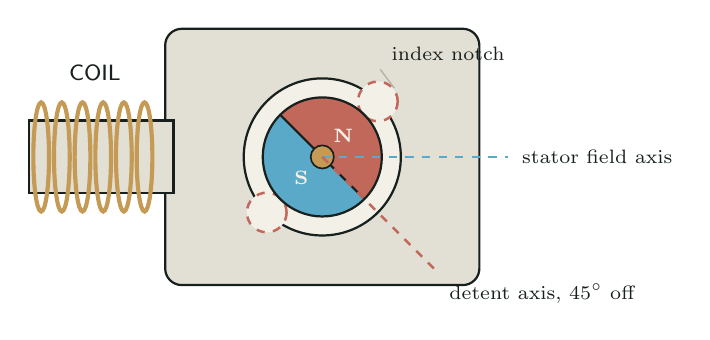
\begin{tikzpicture}[font=\footnotesize\sffamily,scale=1.05]
% stator body with bore (even-odd fill)
\fill[even odd rule,paper!72!rule,draw=ink,line width=.8pt,rounded corners=6pt]
  (-1.6,-1.55) rectangle (2.2,1.55);
\fill[paper!72!rule,draw=ink,line width=.8pt] (-3.25,-0.44) rectangle (-1.5,0.44);
\fill[paper,draw=ink,line width=.8pt] (0.3,0) circle (0.95);
% coil turns around the arm
\foreach \x in {-3.10,-2.85,...,-1.85}{\draw[gold,line width=1.5pt] (\x,0) ellipse (0.095 and 0.66);}
% index notches on the bore
\fill[paper,draw=hot,line width=.9pt,dashed] ({0.3+0.95*cos(45)},{0.95*sin(45)}) circle (0.24);
\fill[paper,draw=hot,line width=.9pt,dashed] ({0.3+0.95*cos(225)},{0.95*sin(225)}) circle (0.24);
% rotor, magnetic axis on the detent axis (45 degrees below horizontal)
\begin{scope}[shift={(0.3,0)},rotate=-45]
  \fill[hot] (0.72,0) arc (0:180:0.72) -- cycle;
  \fill[sig] (-0.72,0) arc (180:360:0.72) -- cycle;
  \draw[ink,line width=.8pt] (0,0) circle (0.72);
  \draw[ink,line width=.8pt] (-0.72,0) -- (0.72,0);
  \node[paper,font=\scriptsize\bfseries] at (0,0.36) {N};
  \node[paper,font=\scriptsize\bfseries] at (0,-0.36) {S};
\end{scope}
\fill[gold,draw=ink,line width=.6pt] (0.3,0) circle (0.14);
% axes
\draw[sig,dashed,line width=.9pt] (0.3,0) -- (2.55,0);
\node[right,ink,font=\scriptsize] at (2.6,0) {stator field axis};
\draw[hot,dashed,line width=.9pt] (0.3,0) -- ++(-45:1.95);
\node[ink,font=\scriptsize,anchor=north west] at (1.72,-1.42) {detent axis, $45^\circ$ off};
\node[ink] at (-2.45,1.02) {COIL};
\node[ink,font=\scriptsize,anchor=south west] at (1.02,1.05) {index notch};
\draw[rule,line width=.5pt] (1.0,1.06) -- ({0.3+0.95*cos(45)+0.2},{0.95*sin(45)+0.16});
\end{tikzpicture}
\caption{Cross-section. Two index notches in the bore saturate locally and rotate the rotor's
rest orientation about $45^\circ$ away from the stator field axis. Without them the rotor would
rest exactly on the field axis, a pulse would produce zero starting torque, and the direction of
rotation would be undefined: a dead centre.}
\end{figure}

\subsection{Torque, and why the step succeeds}

Take $\theta$ from the rest position, positive in the direction of travel. The detent (cogging)
torque has period $180^\circ$ because the rotor is bipolar; the coil torque pulls the rotor
towards the field axis, which the notches have placed at $\theta = 135^\circ$. Writing $J$ for
the rotor inertia and $b$ for damping,
\begin{equation}
J\ddot{\theta} \;=\; \underbrace{-\,T_c \sin 2\theta}_{\text{detent}}
\;+\; \underbrace{T_m \sin(135^\circ - \theta)\,\Pi_{[0,t_p]}(t)}_{\text{coil pulse}}
\;-\; b\dot{\theta}.
\label{eq:lavet}
\end{equation}

\begin{figure}[htbp]
\centering
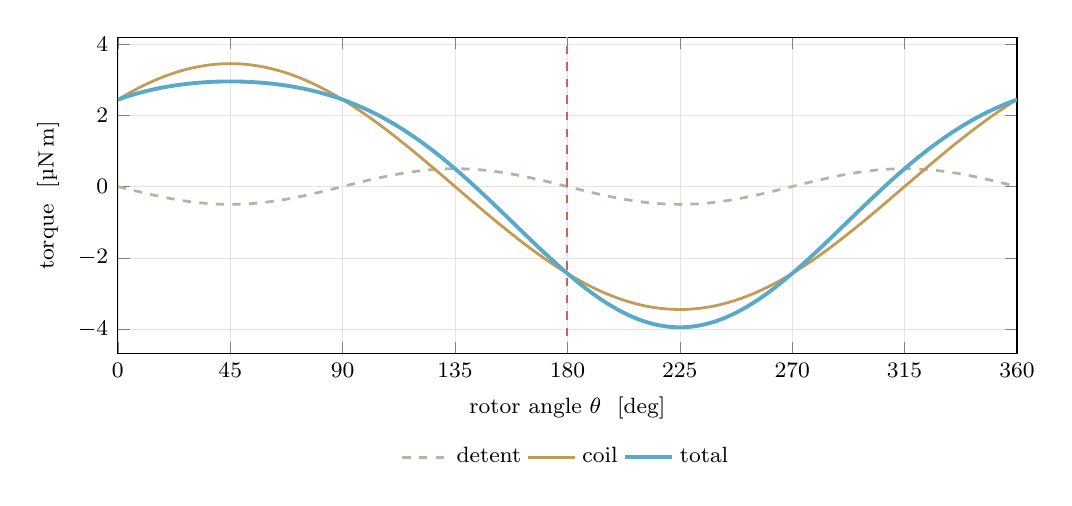
\begin{tikzpicture}
\begin{axis}[
  width=13cm,height=5.6cm,
  xlabel={rotor angle $\theta$ \ [deg]},ylabel={torque \ [\si{\micro\newton\metre}]},
  xmin=0,xmax=360,xtick={0,45,90,135,180,225,270,315,360},
  grid=major,grid style={rule!35,very thin},
  tick label style={font=\footnotesize},label style={font=\footnotesize},
  every axis plot/.append style={line width=1pt},
  legend style={font=\footnotesize,draw=none,fill=none,at={(0.5,-0.26)},anchor=north},
  legend columns=3]
  \addplot[rule,dashed,samples=400,domain=0:360]{-0.5*sin(2*x)};
  \addlegendentry{detent}
  \addplot[gold,samples=400,domain=0:360]{3.45*sin(135-x)};
  \addlegendentry{coil}
  \addplot[sig,line width=1.4pt,samples=400,domain=0:360]{-0.5*sin(2*x)+3.45*sin(135-x)};
  \addlegendentry{total}
  \draw[hot,line width=.7pt,dashed] (axis cs:180,-4.2) -- (axis cs:180,4.2);
\end{axis}
\end{tikzpicture}
\caption{Torque against rotor angle during the pulse, with $T_c = \SI{0.5}{\micro\newton\metre}$
and $T_m = \SI{3.45}{\micro\newton\metre}$. The coil pushes the rotor the whole way past
$90^\circ$; beyond that the detent torque itself changes sign and carries the rotor into the
next stable position at $180^\circ$.}
\end{figure}

Integrating \eqref{eq:lavet} with $J = \SI{2e-12}{\kilogram\metre\squared}$,
$b = \SI{2e-9}{\newton\metre\second}$, $t_p = \SI{4.9}{\milli\second}$ gives a step that
completes in about \SI{6}{\milli\second}, overshoots slightly, and rings down into the detent
well over the following \SI{20}{\milli\second}. The interesting behaviour is at the edges of the
parameter space: shorten the pulse or weaken the drive and the rotor fails to clear the
$90^\circ$ barrier, falling back to where it started; overdrive it and the rotor overruns to
$360^\circ$ and the seconds hand jumps two.

\begin{keybox}
\textbf{Adaptive drive.} Because the failure boundary is sharp, modern ICs cut the pulse short,
then sense the rotor's own back-EMF to confirm it moved. If the step landed, the next pulse is
trimmed shorter still; if it failed, a full-power correction pulse fires immediately. The motor
therefore runs permanently a few percent above its own failure threshold, which is where the
battery life comes from.
\end{keybox}

\subsection{Why the polarity alternates}

After one step the rotor has turned $180^\circ$, so the same field polarity would push it
backwards. Reversing the pulse each second restores the geometry, and the bonus is zero net DC
through the coil: no electrolytic corrosion and no progressive demagnetisation of the rotor.

Chopping the pulse gives the current budget. With the coil at \SI{2}{\kilo\ohm} across
\SI{1.55}{\volt} the peak is \SI{775}{\micro\ampere}; at a \SI{15}{\percent} chopper duty the
mean during the pulse is \SI{116}{\micro\ampere}, the energy per step is about
\SI{0.88}{\micro\joule}, and the average contribution is \SI{0.57}{\micro\ampere}.

% ==================================================================
\section{The train, running backwards}

A mechanical watch gears \emph{up}, from a slow barrel to a fast escapement. A quartz watch
gears \emph{down}, from a fast rotor to slow hands. Same wheels, opposite errand.

\begin{table}[htbp]
\centering
\caption{A representative reduction from rotor to hour hand. The overall ratio is
$30 \times 60 \times 12 = \num{21600}$ to one, and there is no escapement anywhere in the chain.}
\begin{tabular}{@{}llll@{}}
\toprule
Wheel & Speed & Carries & Note \\
\midrule
Rotor            & \SI{30}{\rpm} mean       & \textemdash{}            & half a turn per second \\
Intermediate     & \SI{6}{\rpm}             & \textemdash{}            & first reduction \\
Fourth wheel     & \SI{1}{\rpm}             & seconds hand   & $6^\circ$ per step \\
Third wheel      & \textemdash{}                     & \textemdash{}            & transmission \\
Centre / cannon  & 1 turn per hour         & minute hand    & \\
Hour wheel       & 1 turn per 12 hours     & hour hand      & motion work, $12{:}1$ \\
\bottomrule
\end{tabular}
\end{table}

The visible signature is the tick. A quartz seconds hand advances $6^\circ$ once a second
because the rotor makes exactly half a turn per second and the train divides by sixty. The
``sweep'' of a mechanical watch is really \num{28800} tiny steps an hour, also discrete, just
below the threshold at which the eye separates them.

The structural point is deeper than the aesthetics. In a mechanical watch the train sits
\emph{inside} the timing loop: friction and torque variation reach the balance and change the
rate. In a quartz watch the train is strictly downstream. Gum it up and the hands stop, but
until they do they are never \emph{late}. The loads involved are trivial, roughly a microjoule
per second, so pivots need no jewelling for wear and wheels are often moulded polymer. The
engineering difficulty moved upstream into the silicon.

% ==================================================================
\section{What is left to go wrong}

An XY-cut tuning fork has a parabolic frequency--temperature characteristic with its turnover
near \SI{25}{\celsius}:
\begin{equation}
\frac{\Delta f}{f} \;=\; -\,\beta\,(T - T_0)^2 ,
\qquad \beta \approx \SI{0.035}{\ppm\per\celsius\squared},\ T_0 \approx \SI{25}{\celsius}.
\label{eq:parab}
\end{equation}

\begin{figure}[htbp]
\centering
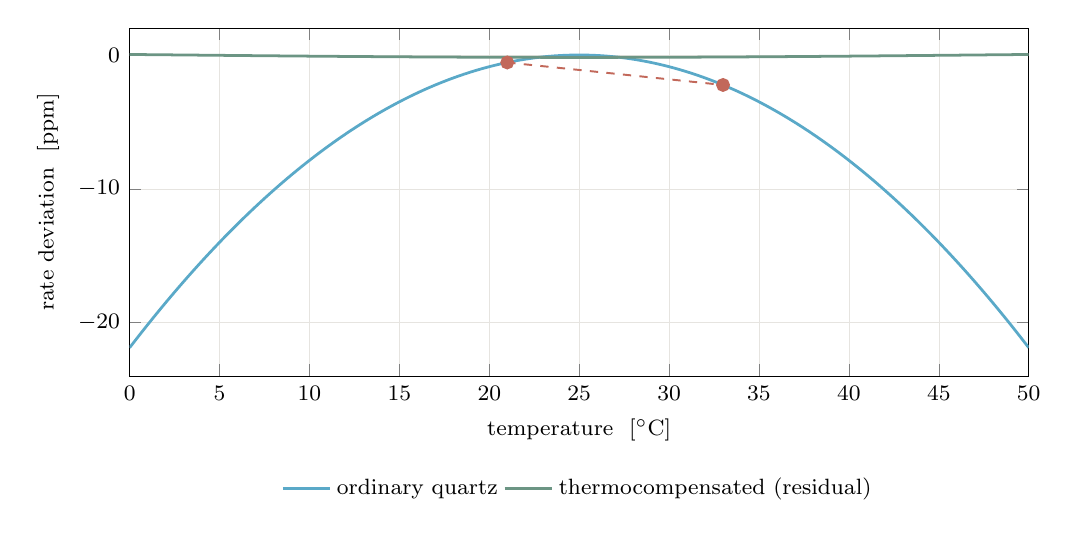
\begin{tikzpicture}
\begin{axis}[
  width=13cm,height=6cm,
  xlabel={temperature \ [\si{\celsius}]},ylabel={rate deviation \ [ppm]},
  xmin=0,xmax=50,ymin=-24,ymax=2,
  grid=major,grid style={rule!35,very thin},
  tick label style={font=\footnotesize},label style={font=\footnotesize},
  every axis plot/.append style={line width=1pt},
  legend style={font=\footnotesize,draw=none,fill=none,at={(0.5,-0.26)},anchor=north},legend columns=2]
  \addplot[sig,samples=200,domain=0:50]{-0.035*(x-25)^2};
  \addlegendentry{ordinary quartz}
  \addplot[mint!60!deep,samples=200,domain=0:50]{-0.18*cos((x-25)/14 r)};
  \addlegendentry{thermocompensated (residual)}
  \addplot[only marks,mark=*,mark size=2pt,hot] coordinates {(21,-0.56) (33,-2.24)};
  \draw[hot,dashed,line width=.7pt] (axis cs:21,-0.56) -- (axis cs:33,-2.24);
\end{axis}
\end{tikzpicture}
\caption{The whole error budget of an ordinary quartz watch, in one curve. The two marked
points are a typical duty cycle, \SI{14}{\hour} on a \SI{33}{\celsius} wrist and
\SI{10}{\hour} on a \SI{21}{\celsius} desk, which average to about \SI{-1.5}{\ppm}, or
\SI{-4}{\second} a month.}
\end{figure}

Note that the parabola opens \emph{downward}, so every departure from the turnover makes the
watch run slow. This is why ordinary quartz watches, as a class, lose rather than gain.

\subsection{Trimming by deletion}

You cannot economically make a crystal that is exactly \SI{32768.000}{\hertz}. Instead the
crystal is deliberately left running slightly fast, and once a minute the IC \emph{deletes} a
small number of counted pulses. One pulse per minute out of $32768 \times 60$ is
\begin{equation}
\frac{1}{32768 \times 60} = \SI{0.51}{\ppm} \approx \SI{1.3}{\second\per\mnth},
\end{equation}
which is the adjustment resolution. Because the trim lives in the digital domain, the
adjustment itself cannot drift.

Thermocompensated movements close the loop: a temperature sensor is sampled every ten to sixty
seconds and the inhibition count is indexed to the measured temperature. The parabola is a
known, stable, per-crystal curve, so it can be cancelled almost entirely. What remains is
ageing, roughly \SIrange{1}{2}{\ppm} in the first year and less thereafter, caused by stress
relaxation in the mount and mass transfer on the tines.

% ==================================================================
\section{Two ways to divide a second}

\begin{figure}[htbp]
\centering
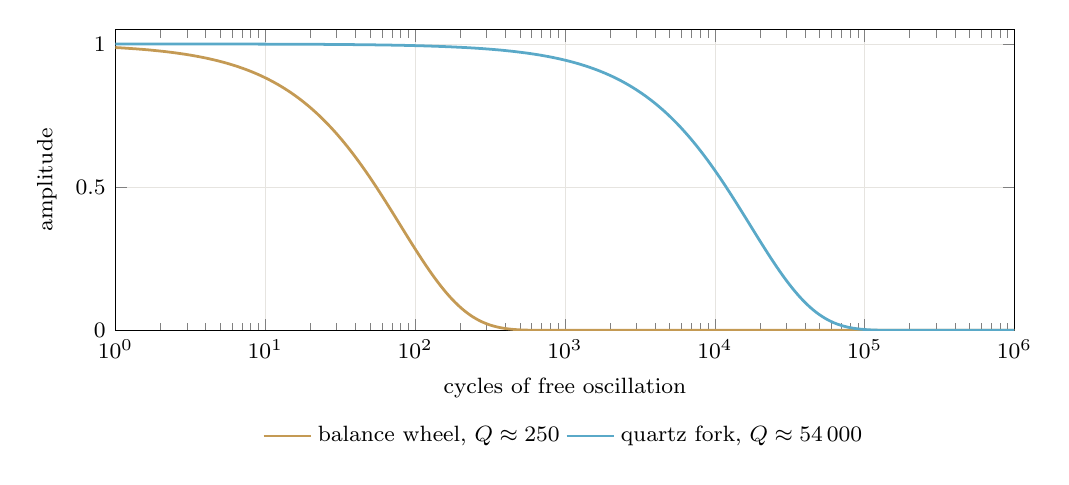
\begin{tikzpicture}
\begin{semilogxaxis}[
  width=13cm,height=5.4cm,
  xlabel={cycles of free oscillation},ylabel={amplitude},
  xmin=1,xmax=1e6,ymin=0,ymax=1.05,
  grid=major,grid style={rule!35,very thin},
  tick label style={font=\footnotesize},label style={font=\footnotesize},
  every axis plot/.append style={line width=1pt},
  legend style={font=\footnotesize,draw=none,fill=none,at={(0.5,-0.28)},anchor=north},legend columns=2]
  \addplot[gold,samples=300,domain=1:1e6]{exp(-pi*x/250)};
  \addlegendentry{balance wheel, $Q \approx 250$}
  \addplot[sig,samples=300,domain=1:1e6]{exp(-pi*x/54000)};
  \addlegendentry{quartz fork, $Q \approx \num{54000}$}
\end{semilogxaxis}
\end{tikzpicture}
\caption{Free ring-down. $Q$ counts the radians of oscillation a resonator keeps before losing
$1/e$ of its energy, which is the same thing as how hard it is to talk out of its own
frequency.}
\end{figure}

For a resonator perturbed by a phase error $\varphi$ per cycle (friction, an off-centre
impulse, a change in position) the fractional rate error scales as
\begin{equation}
\frac{\delta f}{f} \;\approx\; \frac{\varphi}{2Q}.
\end{equation}
A quartz fork has roughly two hundred times the $Q$ of a balance wheel, so it converts the same
disturbance into two hundred times less error. Everything else in this document, the
divider, the motor, the trim, is bookkeeping around that single fact.

\begin{table}[htbp]
\centering
\caption{The comparison, end to end.}
\small
\begin{tabularx}{\textwidth}{@{}l>{\raggedright\arraybackslash}X>{\raggedright\arraybackslash}X>{\raggedright\arraybackslash}X@{}}
\toprule
 & \textbf{Mechanical, chronometer} & \textbf{Quartz, ordinary} & \textbf{Quartz, compensated} \\
\midrule
Timebase        & balance + hairspring & etched quartz fork & fork + temperature sensor \\
Frequency       & \SI{4}{\hertz}, \num{28800}\,vph & \SI{32768}{\hertz} & \SI{32768}{\hertz} \\
Quality factor  & \numrange{200}{300} & $5{\times}10^4$--$10^5$ & $5{\times}10^4$--$10^5$ \\
Rate spec       & $-4/+6$\,s per day & $\pm15$\,s per month & $\pm10$\,s per year \\
Fractional      & ${\approx}5{\times}10^{-5}$ & ${\approx}6{\times}10^{-6}$ & ${\approx}3{\times}10^{-7}$ \\
Dominant error  & position, amplitude, mainspring torque, temperature & the temperature parabola & crystal ageing \\
Regulation      & hairspring length or balance inertia & trimmer capacitor or fixed inhibition & temperature-indexed inhibition \\
Energy          & mainspring, ${\sim}\SI{40}{\hour}$, wrist-wound & \SI{25}{\milli\ampere\hour} cell, 2--3 years & cell, 5--10 years \\
Train's role    & inside the timing loop & downstream only & downstream only \\
Failure mode    & drifts, then stops & keeps perfect time, then stops dead & keeps perfect time, then stops dead \\
\bottomrule
\end{tabularx}
\end{table}

\subsection*{Two hybrids}

Seiko's Kinetic replaces the battery with a rotor-driven generator but keeps the quartz
timebase. Spring Drive keeps the mainspring, barrel and gear train of a mechanical watch and
deletes only the escapement, replacing it with an electromagnetically braked glide wheel that a
quartz oscillator holds to exactly eight turns per second, which is why its seconds hand
genuinely sweeps.

\vspace{6mm}
\begin{center}
\rule{0.4\textwidth}{0.6pt}
\end{center}
\vspace{2mm}

\noindent\emph{An escapement is an analogue negotiation: energy goes in, the balance answers
with an interval, and every imperfection in the negotiation shows up as rate. A quartz watch
removes the negotiation. The crystal decides the interval alone, in a domain where a divider
can be exact and a trim can be an integer. What is left for the mechanism to do is to spend one
pulse a second turning a magnet.}

\end{document}
